\documentclass[aspectratio=43,10pt,spanish]{beamer}
% TODO: sacar tb en 16:9
% \documentclass[aspectratio=169,10pt,spanish]{beamer}


% Idioma
\usepackage[utf8]{inputenc}
\usepackage[T1]{fontenc}
\usepackage[spanish]{babel}
\selectlanguage{spanish}

% Tema
\usetheme{metropolis}

% Notas
\usepackage{pgfpages}
%\setbeameroption{hide notes} % Only slides
%\setbeameroption{show only notes} % Only notes
\setbeameroption{show notes on second screen=right} % Both
\setbeamertemplate{note page}{\pagecolor{yellow!5}\insertnote}\usepackage{palatino}

% Otros
% \usepackage{appendixnumberbeamer} TODO: usar si se añaden referencias
\usepackage{booktabs} % tabular

% Comandos
\let\emph\relax
\newcommand{\emph}{\alert}
%\DeclareTextFontCommand{\emph}{\color{orange!100}}

% Estilos de teoremas
\theoremstyle{definition} % titulo negrita, cuerpo en recta
\newtheorem{teorema}{Teorema}[section]
\newtheorem{proposicion}{Proposicion}[section]
\newtheorem{lema}{Lema}[section]
\newtheorem{ejemplo}{Ejemplo}[section]
\newtheorem{definicion}{Definición}[section]
\newtheorem{nota}{Nota}[section]

\title{Curvas Elípticas en Criptografía}
\subtitle{Trabajo Fin de Grado}
\date{\today}
\author{Adrián H. Ranea Robles}
\institute{Universidad de Granada}

\begin{document}

\maketitle

\begin{frame}{Tabla de contenidos}
    % Hablar algo de se va a seguir el mismo orden de la memoria
    \setbeamertemplate{section in toc}[sections numbered]
    \tableofcontents[hideallsubsections]
\end{frame}

% Hablar un poco de que se va a ver.
\section{Desarrollo matemático}

\begin{frame}{Definición de curva elíptica}
    Sea $K$ un cuerpo. Una \emph{curva elíptica} $E$ se define por una ecuación de la forma
    \begin{align}\label{eq:Weierstrass general}
        E : y^2 = x^3 + a x^2 + b
    \end{align}
    donde $a, b \in K$ y $-16(4a^3 + 27b^2) \neq 0$.

    \vfill

    Denotamos por $E(K)$ al conjunto de pares $(x, y) \in K \times K$ que verifican~\eqref{eq:Weierstrass general} más un punto adicional $\infty$.
    % $$ \{\infty\} \cup \{(x, y) \in K \times K \mid y^2 = x^3 + a x^2 + b \} $$

    \note[item]{ (1) ecuación de Weirstrass }
    \note[item]{ $-16(4a^3 + 27b^2)$ discriminante }
    \note[item]{ Se pide discriminante != 0 para que la curva no tenga puntos singulares. Por ejemplo, para evitar puntos con 2 o más rectas tangentes.}

    \note[item]{ $\infty$ es el punto del infinito}
    \note[item]{ En este caso, veremos a $\infty$ como un punto especial con una serie de propiedades técnicas.}
    \note[item]{ Sin embargo, y como se explica en la memoria, este punto de la recta del infinito (el subconjunto del espacio proyectivo) que satisface la forma proyectiva de la ecuación de Weierstrass. Esto se explica detalladamente en la memoria.}

    \note[item]{ Existe una versión más general de la definición de curva eliptica, que viene dada por una ecuación con 5 coeficientes.}
    \note[item]{ Tal y como hemos comentado en la memoria, si el cuerpo tiene caracteristica distinta de 2 y 3, la ecuación general se puede simplificar a (1) mediate un cambio de variables válido. Para 2 y 3, las ecuaciones simplificadas son distintas.}
    \note[item]{ En esta presentación supondremos que char(K) = 2, 3. En la memoria se estudia también para char(K) = 2, ya que los cuerpos finitos de caracteristica 2 son interesantes en computación.}
\end{frame}

\begin{frame}{Ejemplos de curvas elípticas sobre $\mathbb{R}$}
    \note{ Dos curvas elípticas sobre R cuyas formas son muy ejemplares }
    %\begin{exampleblock}{Curvas elípticas sobre $\mathbb{R}$}
        \begin{columns}[T,onlytextwidth]
            \column{0.5\textwidth}
            \begin{center}
                \includegraphics[width=.9\linewidth]{Graficos/grafo_curva_eliptica_reales_1.pdf}

                $y^2 = x^3 - x$
            \end{center}

            \column{0.5\textwidth}
            \begin{center}
                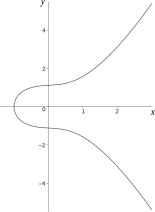
\includegraphics[width=.9\linewidth]{Graficos/grafo_curva_eliptica_reales_2.pdf}

                $y^2 = x^3 + x$
            \end{center}
        \end{columns}
    %\end{exampleblock}
\end{frame}

\begin{frame}{Versión geométrica del método de la cuerda y la tangente}
    %\begin{exampleblock}{}
        \begin{columns}[T,onlytextwidth]
            \column{0.5\textwidth}
            \begin{center}
                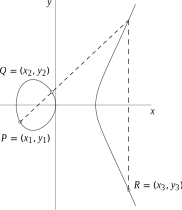
\includegraphics[width=0.8\linewidth]{Graficos/ejemplo_adiccion.pdf}
            \end{center}

            \column{0.5\textwidth}
            \begin{center}
                \includegraphics[width=0.8\linewidth]{Graficos/ejemplo_duplicacion.pdf}
            \end{center}
        \end{columns}
    %\end{exampleblock}

    \vfill

    %\metroset{block=fill}
    \uncover<2>{
        \begin{teorema}
            $(E(K), +, \infty)$ es un grupo abeliano.
        \end{teorema}
    }

    \note[item]{ Veamos como dotar de estructura de grupo al conjunto de puntos de una curva elíptica. Para ello definiremos un ley de composición mediante fórmulas algebraicas. Estas formulas están inspiradas en el siguiente método.}
    \note[item]{	Dados dos puntos $P$ y $Q$ , veamos como producir un tercer punto $R$. En primer lugar si $P$ y $Q$ son distintos, los pasos son:
	\begin{enumerate}
		\item Se dibuja una recta $L$ de $P$ a $Q$.
		\item Esta recta intersecta la curva elíptica en un tercer punto.
		\item Tomamos $R$ como la reflexión de este punto sobre el eje-$x$.
	\end{enumerate}
	Si los puntos $P$ y $Q$ son iguales, los pasos son:
	\begin{enumerate}
		\item Se dibuja la línea tangente $L$ a la curva elíptica en $P$.
		\item Esta línea intersecta la curva elíptica en un segundo punto.
		\item Tomamos $R$ como la reflexión de este punto sobre el eje-$x$.
	\end{enumerate}
    }

    \note[item]{Así, este metodo se traduce a formulas algebraicas, se define una operación binaria en el grupo de puntos con dichas formulas  y se prueba... SIGUIENTE!
    }
    \note[item]{ Para cuerpos base con característica 2 o 3, las fórmulas cambian necesariamente. En la memoria se ve la ley de composición para una curva elíptica sobre un cuerpo finito de característica 2.}
\end{frame}

\begin{frame}{Endomorfismos}
\end{frame}

\begin{frame}{Puntos de torsión}
\end{frame}

\begin{frame}{Curvas elípticas sobre cuerpos finitos}
\end{frame}

\begin{frame}{Teorema de Hasse}
\end{frame}


\section{Desarrollo informático}

\begin{frame}{RSA vs ECC}
\end{frame}

\begin{frame}{El problema del logaritmo discreto sobre curvas elípticas}
\end{frame}

\begin{frame}{Parámetros de dominio y pareja de llaves}
\end{frame}

\begin{frame}{ECDH}
\end{frame}


\section{Programa desarrollado: ccepy}

\begin{frame}{Criptografía con Curvas Elípticas con Python}
\end{frame}

\begin{frame}{Herramientas}
\end{frame}

\begin{frame}{Módulos}
\end{frame}

\begin{frame}[plain]
    \hspace*{-11mm}
    % \vspace{3mm}
    \includegraphics[width=\paperwidth]{Graficos/ejemplo_documentacion}
\end{frame}

\section{Cifrado de las páginas de la UGR}

\begin{frame}{Introducción a HTTPS}
\end{frame}

\begin{frame}{Páginas web de la UGR vulnerables}
\end{frame}

\end{document}
